\chapter{Resultados}
\label{champ:results}
\bigskip
\barra
\bigskip
%\textbf{Nota: Este apartado esta siendo traducido del artículo que se presentara en el workshop PDSEC 2014 en el Conrgeso IEEE IPDPS 2014, adicionalmente se complementara con resultados de pruebas en progreso}.\\
El algoritmo Solución Paralela Aleatoria($SPA$) descrito en la Sección \ref{sec:pbiasedrg} y el algoritmo Solución Paralela Híbrida($SPH$) descrito en la Sección \ref{sec:pbiasedrg} se implementaron haciendo uso del API de OpenMP versi\'on 3, las pruebas de estos se realizaron en un equipo de computo con las siguientes características: 16GB de memoria  RAM y un procesador Intel(R) Core(TM) i7 CPU  Extreme Edition con 6 cores(12 con multithreading). Los respectivos versiones  algoritmos secuenciales Solución Aleatoria(SA) descrito en la Sección \ref{sec:smcrg}($SA$) y Solución Híbrida($SH$) descrito en la Sección \ref{sec:hybrid} se probaron en el mismo equipo de computo haciendo uso de un único procesador(core).\\

Con las soluciones $SA$, $SH$, $SPA$ y $SPH$ se pueden construir redes porosas que cumplan tanto $PC$ y las $RG$; sin embargo el ordenamiento y búsqueda de sitios y enlaces se transforma un mayor numero de cálculos para las versiones $SH$ y $SPH$. En las Figura \ref{fig:traslape-a} y \ref{fig:traslape-h}, se muestran los distintos tiempos de construcción para una red porosa de tamaño $L=100$ utilizando y variando el traslape$\Omega$, en ambas figuras podemos observar que conforme el traslape aumenta el tiempo de ejecución también aumenta esto se debe a que tanto en las versiones secuenciales y paralelas el encontrar enlaces que cumplan con las $RG$ para un sitio se vuelve mas complicado lo que se traduce un notable incremento en numero de cálculos.\\

Comparando las versiones $SA$ y $SPA$ se puede ver en la Figura \ref{fig:traslape-a} que $SPA$ comienza a tener un mejor rendimiento en términos de tiempo cuando el traslape es cercano o mayor a $0.1$ esto se debe a que el numero de violaciones a las $RG$ aumenta y por consiguiente el numero de pasos de Monte Carlo para eliminarlas incrementa y es donde al incrementar el numero de hilos comienza a mejorar el rendimiento.\\

Comparando las versiones $SH$ y $SPH$ se puede ver en la Figura \ref{fig:traslape-h} que $SPH$ siempre es mejor en términos de tiempo independientemente de valor del traslape esto se debe al procedimiento de sembrado de sitios y asignación de enlaces, lo que permite una mejor distribución del trabajo entre los hilos.\\

\begin{figure}[hbtp]
\centering
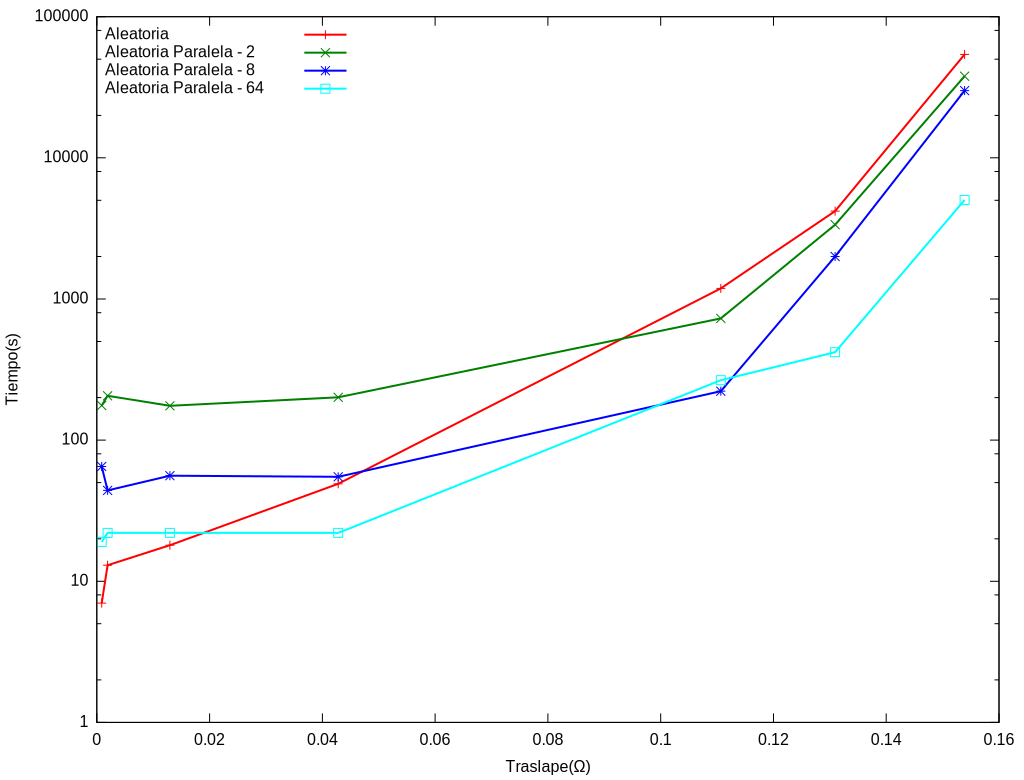
\includegraphics[width=4in]{graphs/traslape_mrg}
\caption{Tiempos de ejecución de $SA$ y $SPA$ utilizando 2,8 y 64 hilos bajo diferentes valores de $\Omega$ (escala logarítmica)}
\label{fig:traslape-a}
\end{figure}

\begin{figure}[hbtp]
\centering
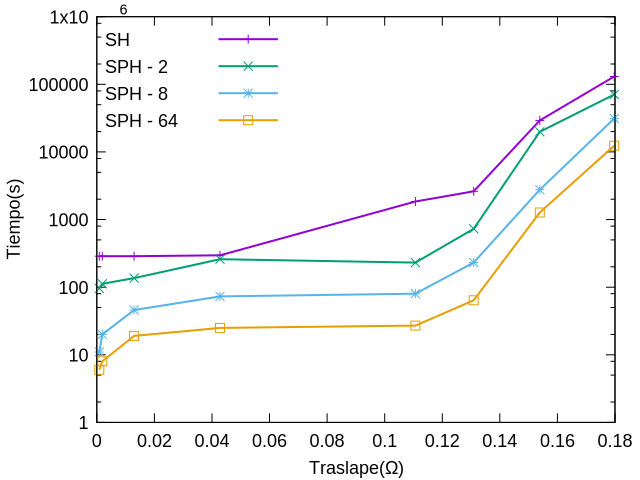
\includegraphics[width=4in]{graphs/traslape_hrg}
\caption{Tiempos de ejecución de $SH$ y $SPH$ utilizando 2,8 y 64 hilos bajo diferentes valores de $\Omega$ (escala logarítmica)}
\label{fig:traslape-h}
\end{figure}

Es evidente que el valor del traslape $\Omega$ alcanzado en las redes que consideran el cumplimiento del $PC$ y las $RG$, es relativamente bajo ($\Omega<1$). Este hecho se debe a la restricción impuesta por las restricciones geométricas. Esto último se ilustra en las ecuaciones \ref{eq:eq02} y \ref{eq:eq03}:

\begin{equation}
B_C(R_S) \geq S(R_S)
\label{eq:eq02}
\end{equation}

\begin{eqnarray}
\nonumber \\
B_C(R_S) = & \{\int\limits^{R_S} ... \int\limits_{0} F_B(R_{B1})\; ... \; F_B(R_{BC})dR_{B1} \nonumber \\
& \; \ldots \; dR_{BC} \}^{1/C}
\label{eq:eq03}
\end{eqnarray}

donde $B_C(R_S)$ corresponde al volumen definido por la ecuación \ref{eq:eq03}; esta se relaciona con el conjunto de enlaces que pueden ser conectados a un sitio, evitando al mismo tiempo la existencia de interferencias entre ellos. $S(R_S)$ es la fracción de sitios que son de tamaño $R_S$ o más pequeños.\\

Las ecuaciones \ref{eq:eq02} y \ref{eq:eq03} restringen el valor de traslape como se muestra en \cite{ref5}, ya que la definición matemática de $B_C(R_S)$ impide en si alcanzar valores cercanos a la unidad, es por eso que los valores mostrados del traslape $\Omega<1$.\\

En la Figura \ref{fig:threads}, se muestran cuatro casos de comparación entre las soluciones $SPA$ y $SPH$ en términos del tiempo de construcción de una red porosa de tamaño $L=100$ con distintos traslapes y variando el numero de hilos utilizados para la construcción de la red. En cada caso se añade como referencia dos lineas rectas que representan los tiempos de construcción de la red porosa con el traslape especificado para las soluciones $SA$ y $SH$.\\

En la Figura \ref{fig:threads60}, se muestra el primer caso para construcción de una red de tamaño $L=100$ con un  traslape de $\Omega=0.001908$, la solución $SPH$ muestra en general un mejor rendimiento que $SPA$ sin embargo muestra un bajo rendimiento respecto a $SA$ esto se debe a que al utilizar un traslape tan pequeño el numero de violaciones a las $RG$ es bajo por lo cual la solucion $SPH$ consume la mayor parte de su tiempo en la inicialización de la red particularmente en proceso de ordenamiento de sitios y enlaces mientras que $SA$ trabaja directamente en la eliminación de las violaciones, lo mismo ocurre con $SH$.\\

En la Figura \ref{fig:threads50}, se muestra el segundo caso para construcción de una red de tamaño $L=100$ con un  traslape de $\Omega=0.042809$, podemos ver que $SPA$ y $SPH$ muestran un compartimento muy similar en el cual a partir del uso de mas de 8 hilos mejoran su rendimiento respecto a $SA$, al aumentar el traslape también aumenta el numero de violaciones a las $RG$ lo que se transforma en mayor trabajo para cada hilo. Para $SPA$ en el caso anterior y en el actual(hasta 8 hilos) la mayor parte de tiempo se consumía en la distribución y redistribución de los datos es por eso que se muestra un rendimiento menor que $SA$. Para $SPH$ por las mismas causas tiene que un compartimento similar al del caso  sin embargo en este caso se obtuvo un recudimento mejor que el de $SA$ utilizando 8 hilos a diferencia de los 32 necesarios en el caso anterior.\\

En la Figura \ref{fig:threads43}, se muestra el tercer caso para construcción de una red de tamaño $L=100$ con un traslape de $\Omega=0.153895$, la solución $SPH$ muestra un mejor rendimiento que $SA$ y $SPA$ esto como consecuencia de dos factores el primero es que el traslape ocasiono un aumento significativo de violaciones a las $RG$ y el segundo es el proceso de inicializacion que en $SA$ y $SPA$ es completamente aleatorio lo que hace que el numero de violaciones a las $RG$ respecto a $SH$ y $SPH$ sea mucho mayor.\\

En la Figura \ref{fig:threads42}, se muestra el cuarto caso para construcción de una red de tamaño $L=100$ con un traslape de $\Omega=0.179723$, para este valor de traslape los tiempos de ejecución de las soluciones $SA$ y $SPA$ se incrementaron de forma exponencial por lo cual se interrumpió su ejecución. Para $SPH$ se pudo observar que en todos los casos siempre se mantuvo con un mejor rendimiento respecto a $SH$.\\

Adicionalmente en todos los casos mostrados en la Figura \ref{fig:threads}, se utilizaron hasta 64 hilos en las pruebas lo cual supera al numero cores o hilos de ejecución(hyperthreading) disponibles en el equipo de computo donde se realizaron las pruebas, sin embargo esta sobrecarga no efecto de forma negativa el rendimiento de las soluciones $SPA$ y $SPH$ si no al contrario, esto se debe a dos factores el primero es la naturaleza de los algoritmos utilizados en los cuales al particionar y operar sobre los datos no es necesaria una operación de reducción o unión esto da como resultado que la suma del tiempo de trabajar con conjuntos de datos mas pequeños sea menor al tiempo que se necesitaría completar la misma tarea con un conjunto del tamaño de la suma se los conjuntos mas pequeños, el segundo factor es la planificación de los hilos por parte del sistema operativo el cual puede manejar un numero de hilos superior al numero al numero cores o hilos de ejecución(hyperthreading). La mejora en tiempo con sobrecarga se obtuvo de forma constante utilizando hasta 64 hilos, al utilizar una valor mas elevado se comenzaron a tener resultados impredecibles.\\
\vfill
\pagebreak
%65	0.000862
%60	0.001908
%55	0.012969
%50	0.042809
%45	0.110658
%44	0.130928
%43	0.153895
%42	0.179723
\begingroup
\setlength{\parindent}{0cm}
\begin{figure}[hbtp]
\centering
\begin{tabular}{cc}
\subfloat[$\Omega=0.001908$]{
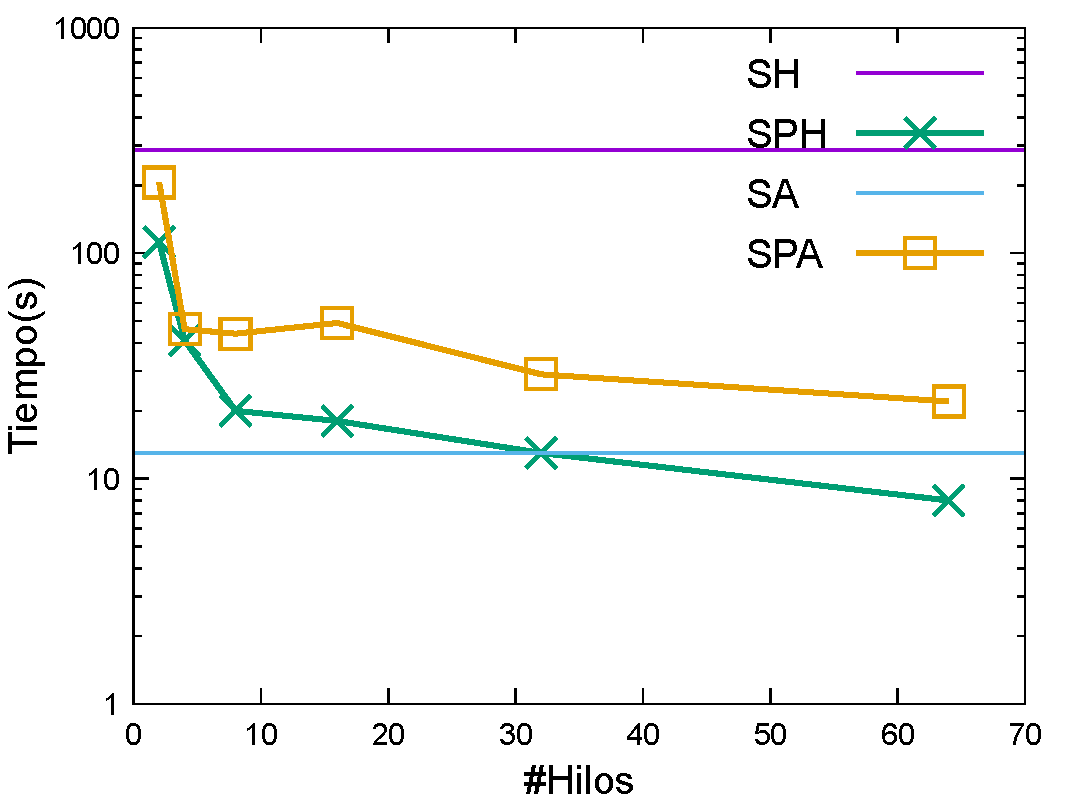
\includegraphics[width=2.7in]{graphs/threads60}
\label{fig:threads60}}
& \subfloat[$\Omega=0.042809$]{
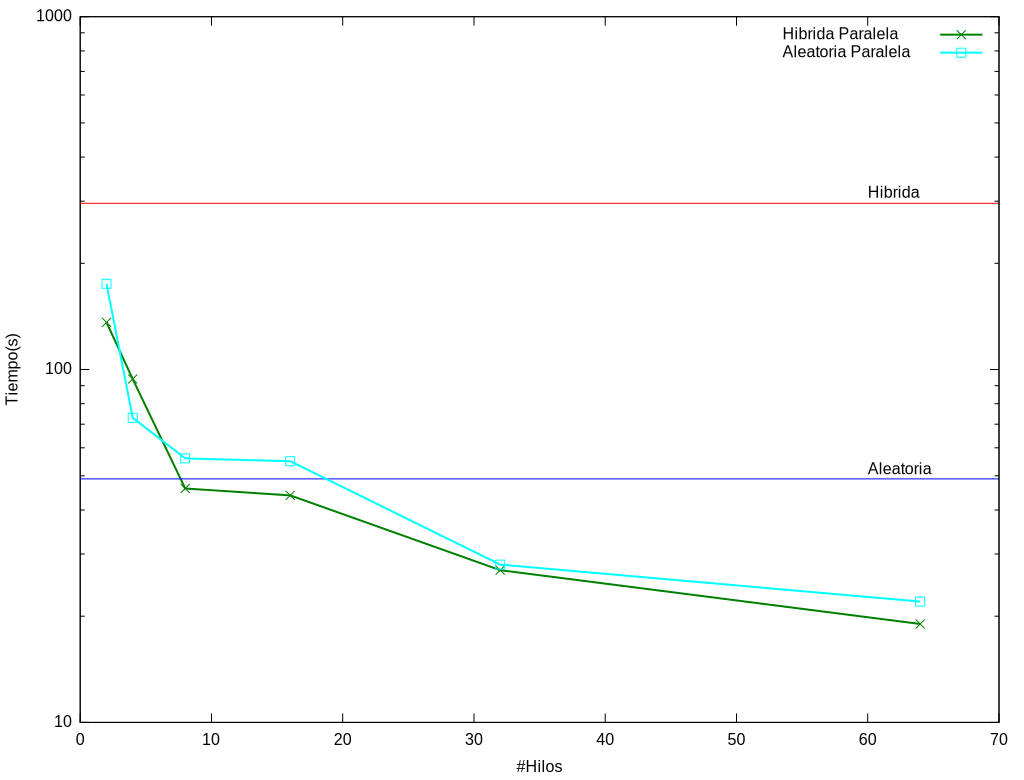
\includegraphics[width=2.7in]{graphs/threads50}
\label{fig:threads50}}\\
\subfloat[$\Omega=0.153895$]{
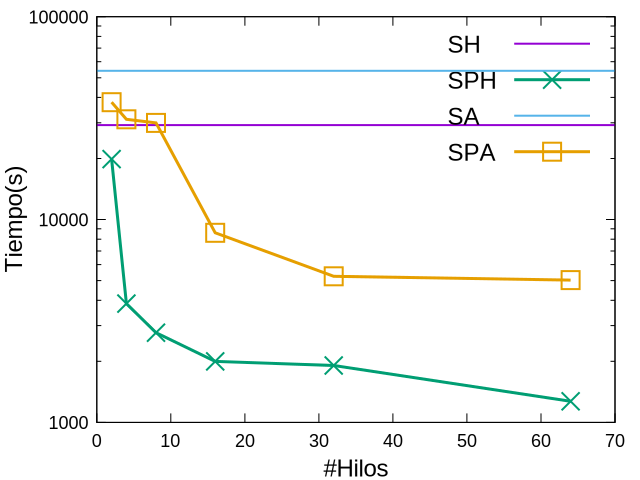
\includegraphics[width=2.7in]{graphs/threads43}
\label{fig:threads43}}
& \subfloat[$\Omega=0.179723$]{
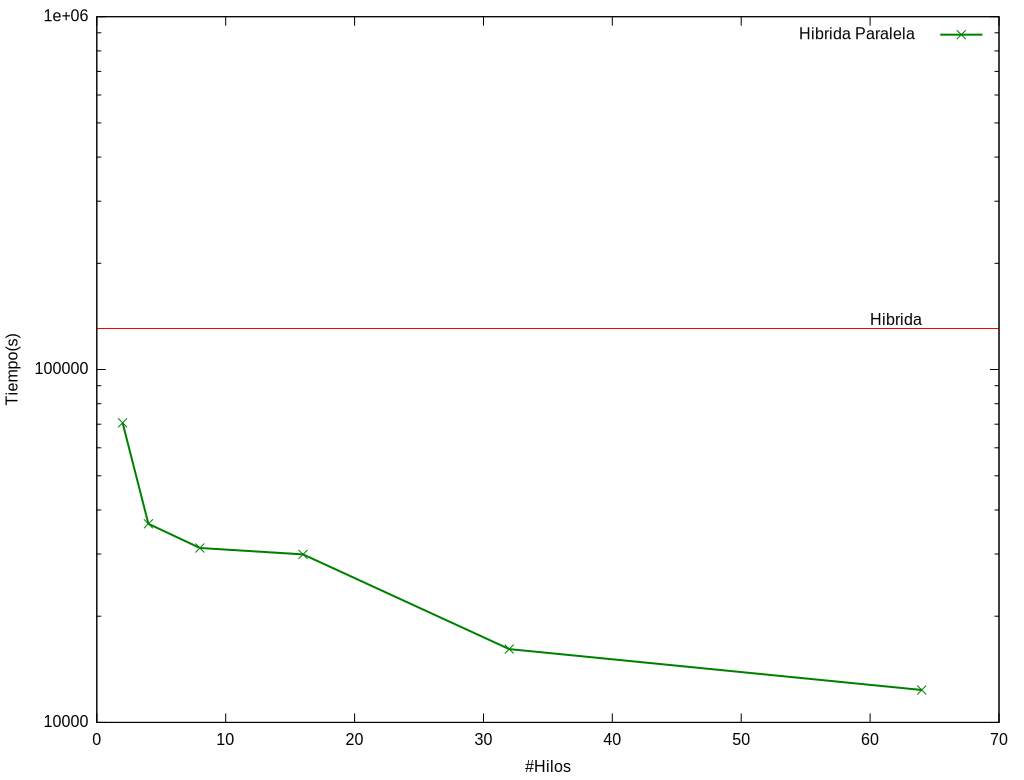
\includegraphics[width=2.7in]{graphs/threads42}
\label{fig:threads45}}
\end{tabular}
\caption{Tiempos de ejecución para $SH$, $SPH$, $SH$ y $SPH$ con distintos traslapes y variando el numero de hilos(escala logarítmica)}
\label{fig:threads}
\end{figure}
\endgroup

\pagebreak
\begin{figure}[hbtp]
\centering
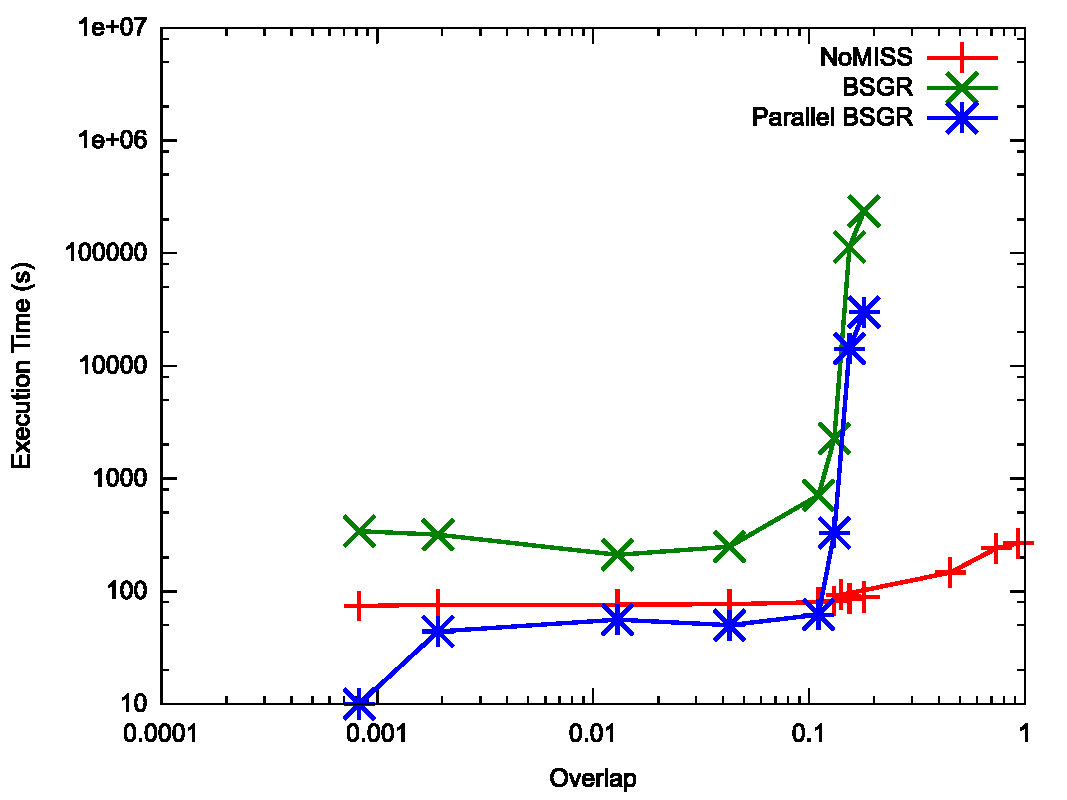
\includegraphics[width=4in]{img/variatraslape.pdf}
\caption{Tiempos de ejecución de NoMISS, BSGR y BSGR paralelo, bajo diferentes valores de $\Omega$ (escala logarítmica)}
\label{fig:timevartraslape}
\end{figure}

La Figura \ref{fig:timenuevo} muestra el timepo de ejecución requerido para crear una red porosa con $L=100$, $\Omega=0.15$, $ClusterSize=32$, y $NClusters=30$ utilizando un número de hilos diferente. El tiempo de ejecución en paralelo en general disminuye mientras aumenta el número de hilos. Podemos observar en algunos casos, como cuando el número e hilos  es igual a 6 y 14, el tiempo de ejecución no disminuye; creemos que estos casos se deben a la siembra aleatoria de clusters lo cual genera un número mayor de violaciones a las $RG$ que en los otros casos, al tener un mayor número de violaciones el tiempo que lleva generar una red porosa válida es mayor.\\
 
\begin{figure}[hbtp]
\centering
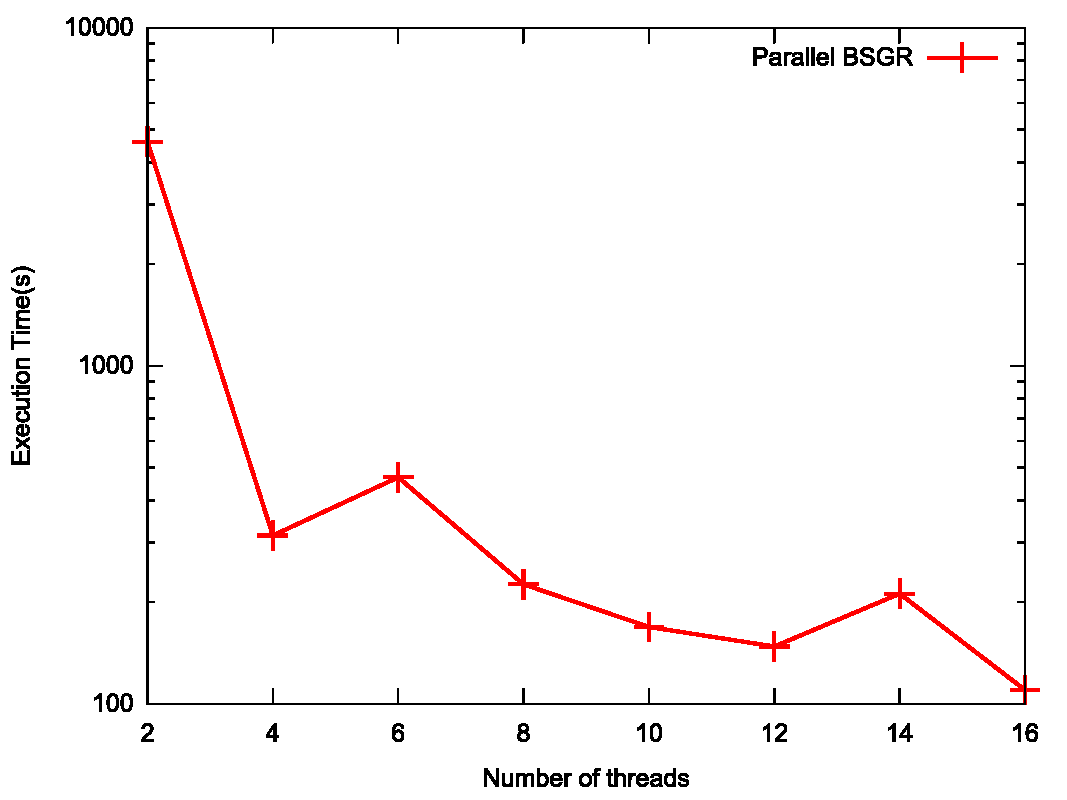
\includegraphics[width=4in]{img/tiempoPar2To16.pdf}
\caption{Tiempos de ejecución de BSGR Paralelo utilizando de 2 a 16 hilos (escala logarítmica)}
\label{fig:timenuevo}
\end{figure}

En la Figura \ref{fig:redes} observamos un ejemplo gráfico de una red porosa con $L=100$ y $\Omega=0.15$, obteniendo a partir de la versión BSGR (Figura \ref{fig:red1}), así como de la versión BSGR Paralela (Figura \ref{fig:red2}) utilizando 8 hilos. Estas imágenes representas redes porosas después del sembrado de cluster de poros y los pasos de asignación de enlaces; es decir, que se permite la existencia de violaciones a las $RG$. El código de color asignado en las Figuras \ref{fig:redes}, \ref{fig:redes2} y \ref{fig:redes3} es como sigue: los poros grandes se muestran de color rojo, los poros de tamaño medio de color azul y los poros pequeños en color azul claro.\\

La Figura \ref{fig:redes2} muestra las anteriores redes porosas después de eliminar por completo las violaciones a las $RG$ a través de la aplicación de $MCs$. En las Figuras \ref{fig:red3} y \ref{fig:red4}, se puede observar que aun quedan estructuras de poro cúbicas que en redes porosas reales no se presentan.\\

Después de aplicar un número adicional de $MCs$ le ísotropia de la red se mejora, obteniendo redes porosas que representan redes porosas más reales, como se muestra en las Figuras \ref{fig:red5} y \ref{fig:red6}.\\

\begin{figure}[hbtp]
\centering
\begin{tabular}{cc}
\subfloat[$ $]{
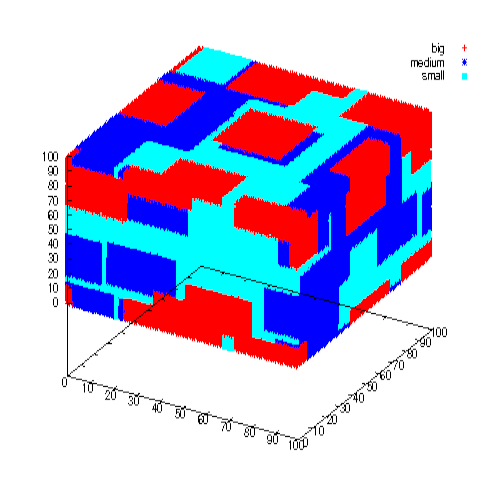
\includegraphics[width=2.3in]{img/redsec100.png}
\label{fig:red1}}
& \subfloat[$ $]{
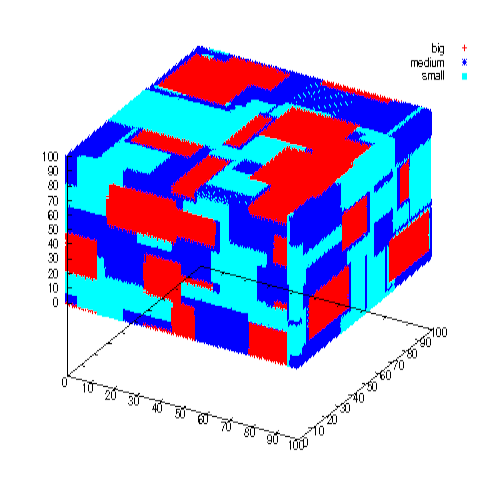
\includegraphics[width=2.3in]{img/redpar100.png}
\label{fig:red2}}
\end{tabular}
\caption{Redes porosas que permiten violaciones a las $GR$, con $L=100$ y $\Omega=0.15$, obtenidas con (a) BSGR y (b) BSGR Paralelo utilizando 8 hilos}
\label{fig:redes}
\end{figure}

\begin{figure}[hbtp]
\centering
\begin{tabular}{cc}
\subfloat[$ $]{
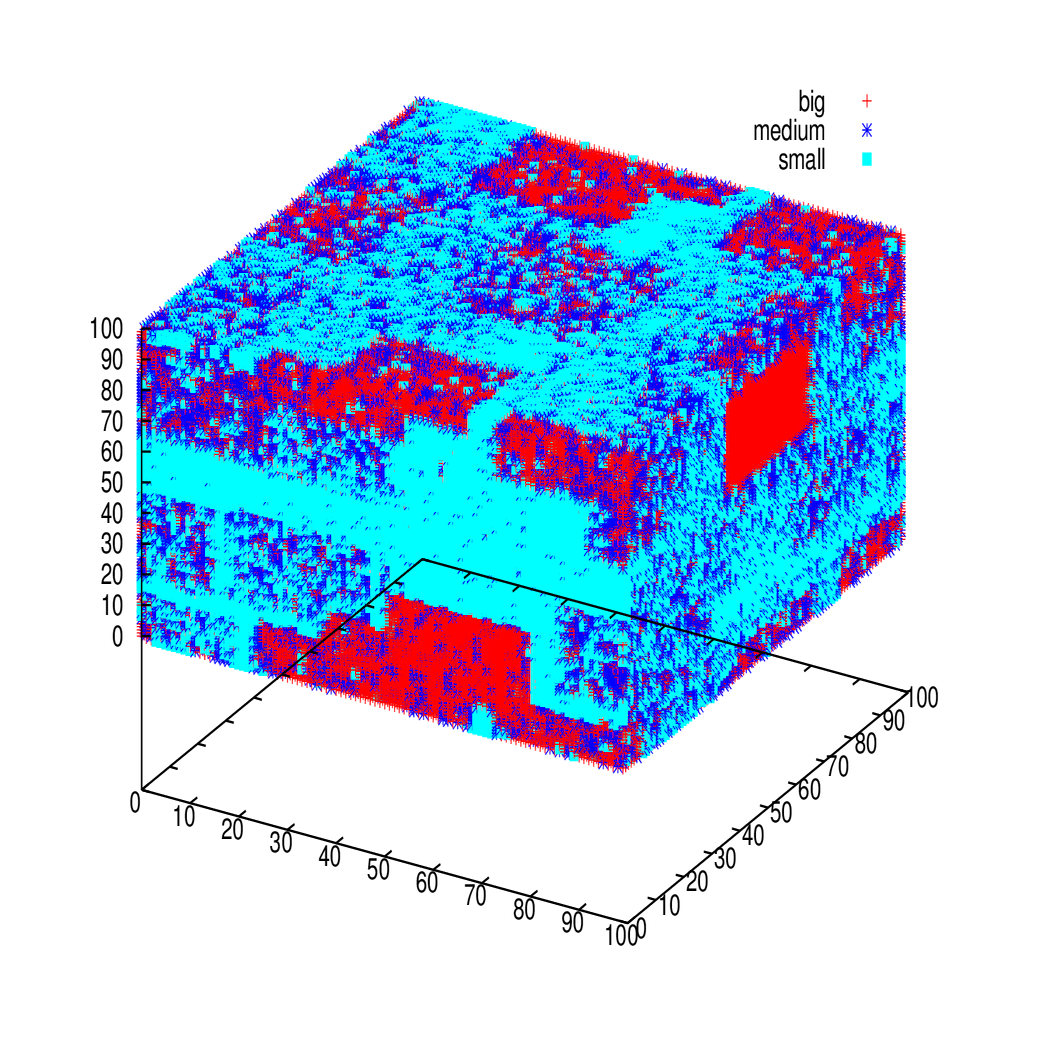
\includegraphics[width=2.3in]{img/red3.png}
\label{fig:red3}}
& \subfloat[$ $]{
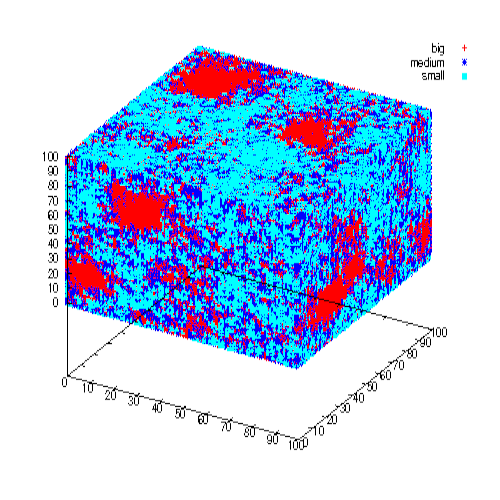
\includegraphics[width=2.3in]{img/red4.png}
\label{fig:red4}}
\end{tabular}
\caption{Redes porosas libre de violaciones a las $GR$, con $L=100$ y $\Omega=0.15$, obtenidas con (a) BSGR  and (b) BSGR Paralelo utilizando 8 hilos}
\label{fig:redes2}
\end{figure}

%\begin{figure}[h]
%\centering
%\begin{tabular}{cc}
%\subfloat[$ $]{
%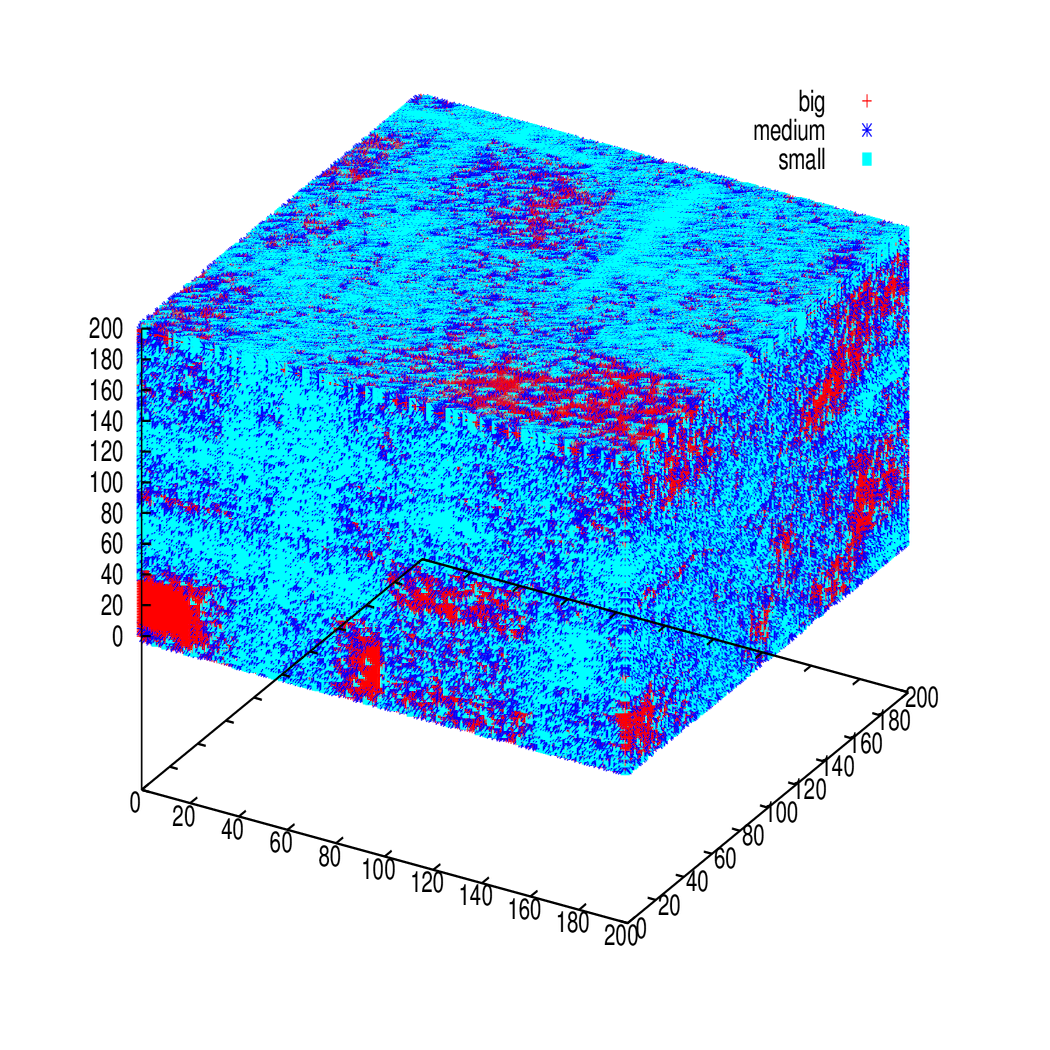
\includegraphics[width=1.5in]{img/red5.png}
%\label{fig:red5}}
%& \subfloat[$ $]{
%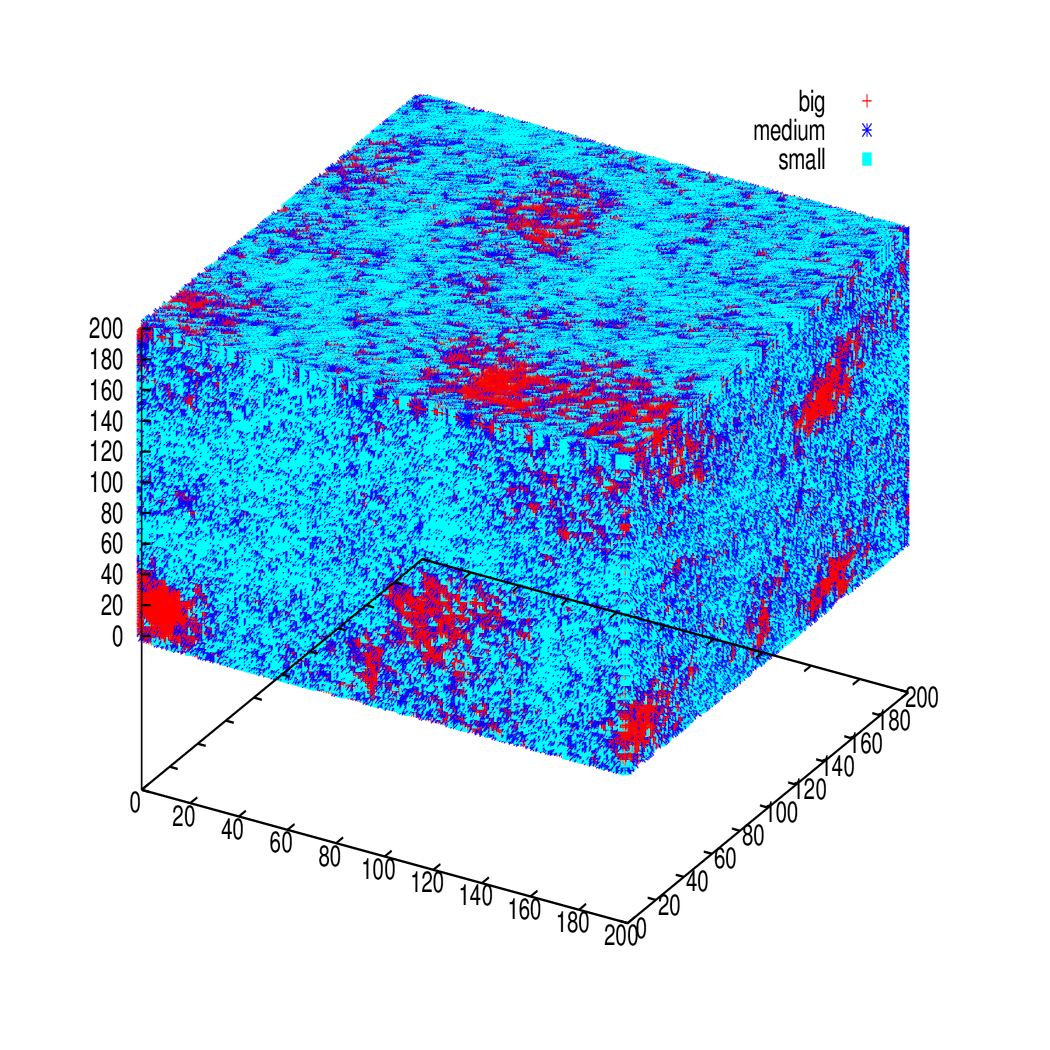
\includegraphics[width=1.5in]{img/red6.png}
%\label{fig:red6}}
%\end{tabular}
%\caption{Pore networks with additional application of $MCs$, obtained from the Parallel BSGR with $L=200$ and $\Omega=0.15$, (a) using 2 threads and (b) using 8 threads}
%\label{fig:redes3}
%\end{figure}

\begin{figure}[t]
\centering
\begin{tabular}{cc}
\subfloat[$ $]{
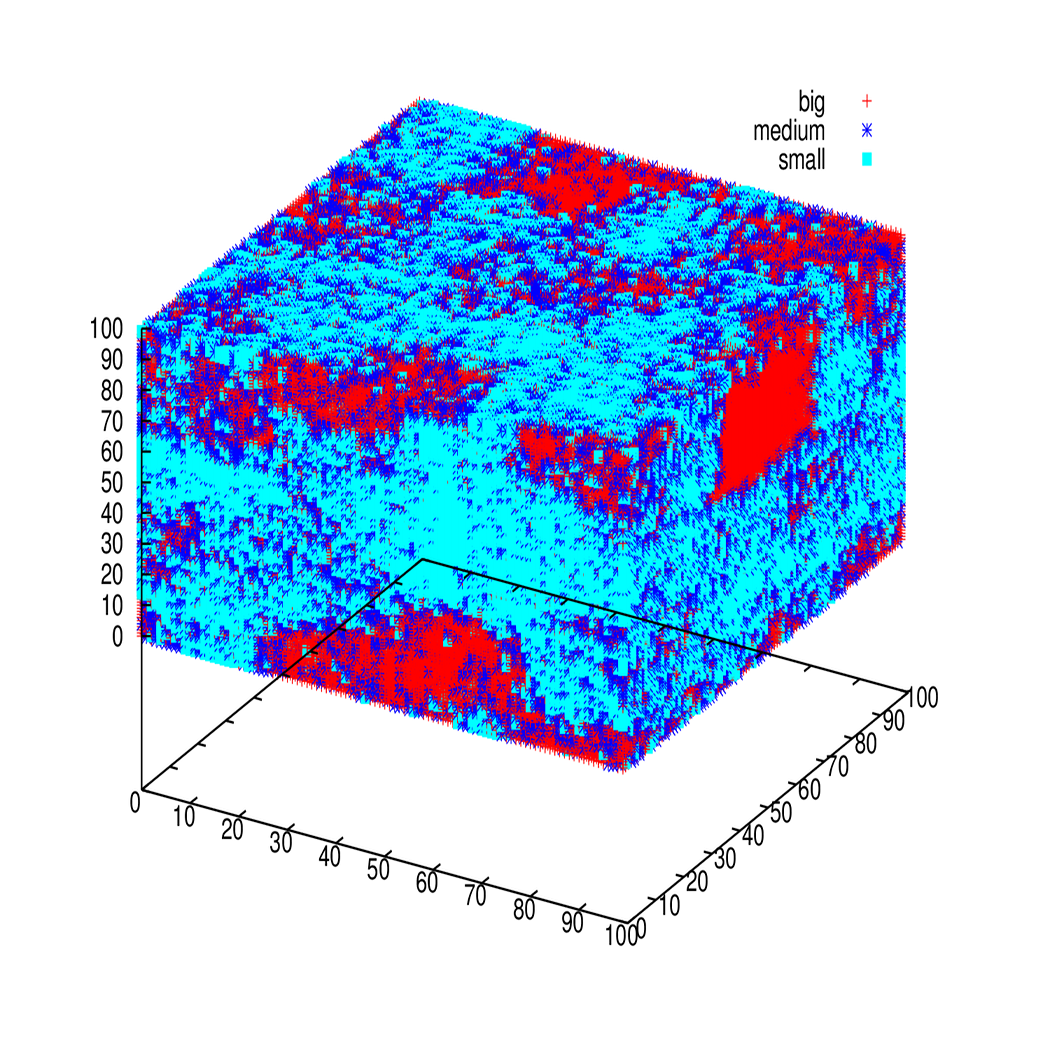
\includegraphics[width=2.3in]{img/red7.png}
\label{fig:red5}}
& \subfloat[$ $]{
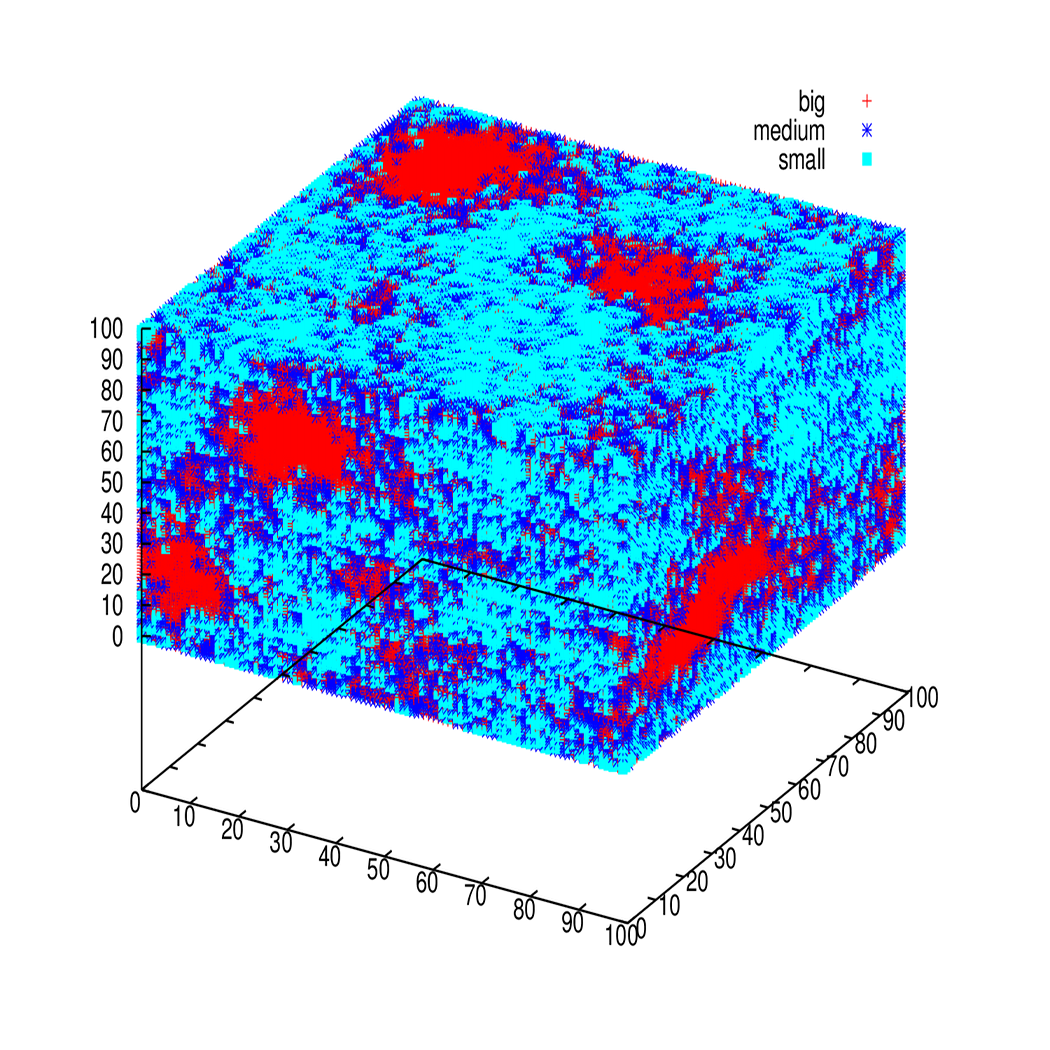
\includegraphics[width=2.3in]{img/red8.png}
\label{fig:red6}}
\end{tabular}
\caption{Redes porosas después de aplicar 2,000 $MCs$ adicionales, con L Pore networks after the application of 2000 additional $MCs$, con $L=100$ y $\Omega=0.15$, obtenidas con (a) BSGR  and (b) BSGR Paralelo utilizando 8 hilos}
\label{fig:redes3}
\end{figure}
